\section{Comparison of Available Wireless Communication Technologies}

There are three ways to communicate wirelessly underwater. These are
acoustic, optical and \ac{RF}.

\begin{figure}[H]
  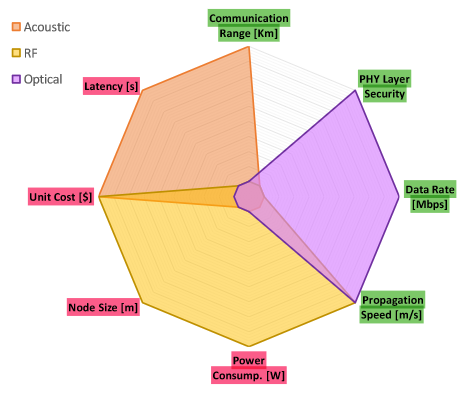
\includegraphics[width=0.8\textwidth]{acoustic_rf_optical_comparison.png}
  \caption{Comparison of Acoustic vs RF vs Optical Technologies}
  \label{fig:acoustic_rf_optical_comparison}
\end{figure}

\subsection{Above Surface to Surface}
This can use RF technologies so is unecessary to consider.

\subsection{Above Surface to Underwater}
A \ac{UAV} communicating with an \ac{ROV} underwater could utilise an optical
link although the surface of the water needs to be taken into account, as well
as the properties under the water.

\subsection{Surface to Underwater}
A ship communicating with an underwater sensor or \ac{ROV} could utilise
optical links to increase bandwidth.

\subsection{Hybrid Approaches}
It is conclusive that hybrid approaches using all available technologies
for their strengths must be the way forward.

\subsubsection{Control Plane versus Data Plane}
It is possible to utilise a hybrid approach to wireless underwater
communications. For example, we can use the much more reliable
acoustic link, which has a much lower data rate, for the control
plane. This gives reliability but a low throughput. The data plane
would then be over the optical link, giving high throughput with
much higher range than \ac{RF}.